% Copyright 2002-2023 The University of Maryland Baltimore County (UMBC)
% 1000 Hilltop Circle, Baltimore, Maryland, 21250, USA
% https://www.csee.umbc.edu/

\documentclass[graphics]{beamer}
\usepackage{graphicx}
\usepackage{listings} % Syntax highlighing
\usepackage{fancyvrb} % Inline verbatim
\usepackage{hyperref} % Hyperlinks
\usepackage{attachfile} % attach files
\hypersetup{pdfpagemode=FullScreen}

\usepackage[normalem]{ulem}               % to striketrhourhg text
\newcommand\redout{\bgroup\markoverwith
{\textcolor{red}{\rule[0.5ex]{2pt}{0.8pt}}}\ULon}

% header in tables
\newcommand*{\thead}[1]{\multicolumn{1}{c}{\bfseries #1}}

% used for arrows from one point in the slide to another
\usepackage{tikz}
\usetikzlibrary{arrows, shapes, tikzmark, positioning}

\newcommand{\backupbegin}{
   \newcounter{framenumberappendix}
   \setcounter{framenumberappendix}{\value{framenumber}}
}
\newcommand{\backupend}{
   \addtocounter{framenumberappendix}{-\value{framenumber}}
   \addtocounter{framenumber}{\value{framenumberappendix}} 
}

\usetheme{Boadilla}
\title{Lecture 16: Functions, Part 3}
\author{UMBC CMSC 104}
\date{Spring 2024}

\begin{document}

\begin{frame}{}
\centering
    Functions, Part 3
\end{frame}

\frame{\tableofcontents}

\begin{frame}{Coding Practice}
    Starting with some simple problems, we will:
    \begin{enumerate}
        \item Design appropriate algorithms
        \item Modularize them
        \item Create pseudocode
        \item Write actual C code
    \end{enumerate}
\end{frame}

\section{Coding Practice: The Box}
\subsection{Problem}
\begin{frame}{The Box}
    \underline{Problem:} Write an interactive program to compute and display the volume and surface area of a box. The program must also display the box dimensions. Error checking should be done to ensure the dimensions are greater than zero.
\end{frame}

\begin{frame}{Hierarchy Chart}
    \centering
    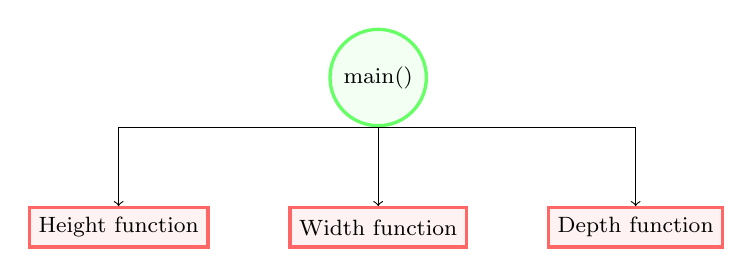
\begin{tikzpicture}[
        roundnode/.style={circle, draw=green!60, fill=green!5, very thick, minimum size=7mm},
        squarednode/.style={rectangle, draw=red!60, fill=red!5, very thick, minimum size=5mm},
        ]
        %Nodes
        \node[squarednode]  (heightfunc)                      {\footnotesize{Height function}};
        \node[squarednode]  (widthfunc) [right=of heightfunc] {\footnotesize{Width function}};
        \node[roundnode]    (mainnode)  [above=of widthfunc]  {\footnotesize{main()}};
        \node[squarednode]  (depthfunc) [right=of widthfunc]  {\footnotesize{Depth function}};
        
        %Lines
        \draw[->] (mainnode.south) -| (heightfunc.north);
        \draw[->] (mainnode.south) -- (widthfunc.north);
        \draw[->] (mainnode.south) -| (depthfunc.north);
    \end{tikzpicture}

    ~~ \\ ~~

    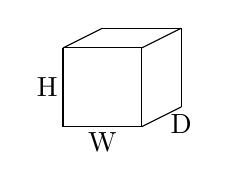
\begin{tikzpicture}
        \draw (0,0) -- (0,1);
        \draw (0,0) -- (1,0);
        \draw (1,0) -- (1,1);
        \draw (0,1) -- (1,1);
        % 3D - top
        \draw (0,1) -- (0.5, 1.25); % top
        \draw (1,1) -- (1.5, 1.25); % top right
        \draw (0.5, 1.25) -- (1.5, 1.25); % top rear
        % 3D - right
        \draw (1,0) -- (1.5, 0.25); % bottom angle
        \draw (1.5, 0.25) -- (1.5, 1.25); % rear vertical
        % Labels
        \node (a) at (-0.2,0.5) {H};
        \node (b) at (0.5,-0.2) {W};
        \node (b) at (1.5,0.03) {D};
    \end{tikzpicture}
\end{frame}

\subsection{Pseudocode}
\begin{frame}[fragile]{The Box - Height Pseudocode}
    \begin{verbatim}
Display "Enter the height: "
Read <height>
While(<height> <= 0)
    Display "The height must be > 0"
    Display "Enter the height: "
    Read <height>
End_while
Return height
    \end{verbatim}
\end{frame}

\begin{frame}[fragile]{The Box - Width Pseudocode}
    \begin{verbatim}
Display "Enter the width: "
Read <width>
While(<width> <= 0)
    Display "The width must be > 0"
    Display "Enter the width: "
    Read <width>
End_while
Return width
    \end{verbatim}
\end{frame}

\begin{frame}[fragile]{The Box - Depth Pseudocode}
    \begin{verbatim}
Display "Enter the depth: "
Read <depth>
While(<depth> <= 0)
    Display "The depth must be > 0"
    Display "Enter the depth: "
    Read <depth>
End_while
Return depth
    \end{verbatim}
\end{frame}

\begin{frame}[fragile]{The Box - Pseudocode (cont'd)}
    \begin{verbatim}
Call height_function saving answer in <height>
Call width_function saving answer in <width>
Call depth_function saving answer in <depth>

<volume> = <height> X <width> X <depth>

<surface1> = <height> X <width>
<surface2> = <width> X <depth>
<surface3> = <height> X <depth>
<surface_area> = 2 X (<surface1> + <surface2> + <surface3>)

Display "Height: ", <height>
Display "Width: ", <width>
Display "Depth: ", <depth>
Display "Volume: ", <volume>
Display "Surface area: ", <surface_area>
    \end{verbatim}
\end{frame}

\subsection{Code the Design}
\begin{frame}[fragile]{Code the Design}
    \begin{lstlisting}[language=C,basicstyle=\footnotesize,keywordstyle=\color{blue},commentstyle=\color{green},showstringspaces=false,stringstyle=\color{red}]
#include <stdio.h>

int height_function();
int width_function();
int depth_function();
    \end{lstlisting}
\end{frame}

\begin{frame}[fragile]{Code the Design}
    \begin{lstlisting}[language=C,basicstyle=\footnotesize,keywordstyle=\color{blue},commentstyle=\color{green},showstringspaces=false,stringstyle=\color{red}]
int main() {
    int height, width, depth, volume;
    int surface1, surface2, surface3, surface_area;
    
    height = height_function();
    width = width_function();
    depth = depth_function();
    
    volume = height * width * depth;
    surface1 = height * width;
    surface2 = width * depth;
    surface3 = depth * height;
    surface_area = 2 * (surface1 + surface2 + surface3);
    
    printf("Height: %d, Width: %d, Depth: %d\n", height,
        width, depth);
    printf("Volume: %d\n", volume);
    printf("Surface area: %d\n", surface_area);
    return 0;
}
    \end{lstlisting}
\end{frame}

\begin{frame}[fragile]{height\_function()}
    \begin{lstlisting}[language=C,basicstyle=\footnotesize,keywordstyle=\color{blue},commentstyle=\color{green},showstringspaces=false,stringstyle=\color{red}]
int height_function() {
    int height;
    printf("Enter the height: ");
    scanf("%d", &height);
    while(height <= 0) {
        printf("The height must be greater than zero!\n");
        printf("Enter the height: ");
        scanf("%d", &height);
    }
    return height;
}
    \end{lstlisting}
\end{frame}

\begin{frame}[fragile]{width\_function()}
    \begin{lstlisting}[language=C,basicstyle=\footnotesize,keywordstyle=\color{blue},commentstyle=\color{green},showstringspaces=false,stringstyle=\color{red}]
int width_function() {
    int width;
    printf("Enter the width: ");
    scanf("%d", &width);
    while(width <= 0) {
        printf("The width must be greater than zero!\n");
        printf("Enter the width: ");
        scanf("%d", &width);
    }
    return width;
}
    \end{lstlisting}
\end{frame}

\begin{frame}[fragile]{depth\_function()}
    \begin{lstlisting}[language=C,basicstyle=\footnotesize,keywordstyle=\color{blue},commentstyle=\color{green},showstringspaces=false,stringstyle=\color{red}]
int depth_function() {
    int depth;
    printf("Enter the depth: ");
    scanf("%d", &depth);
    while(depth <= 0) {
        printf("The depth must be greater than zero!\n");
        printf("Enter the depth: ");
        scanf("%d", &depth);
    }
    return depth;
}
    \end{lstlisting}
\end{frame}

\subsubsection{Easier Way?}
\begin{frame}{Easier Way?}
    \begin{itemize}
        \item Doesn't this seem repetitive?
        \pause
        \item Let's instead pass the name of the variable we want!
    \end{itemize}
\end{frame}

\begin{frame}[fragile]{Code the Design}
    \begin{lstlisting}[language=C,basicstyle=\footnotesize,keywordstyle=\color{blue},commentstyle=\color{green},showstringspaces=false,stringstyle=\color{red}]
#include <stdio.h>

int get_value(char* label);
    \end{lstlisting}
\end{frame}

\begin{frame}[fragile]{Code the Design}
    \begin{lstlisting}[language=C,basicstyle=\footnotesize,keywordstyle=\color{blue},commentstyle=\color{green},showstringspaces=false,stringstyle=\color{red}]
int main() {
    int height, width, depth, volume;
    int surface1, surface2, surface3, surface_area;
    
    height = get_value("height");
    width = get_value("width");
    depth = get_value("depth");
    
    volume = height * width * depth;
    surface1 = height * width;
    surface2 = width * depth;
    surface3 = depth * height;
    surface_area = 2 * (surface1 + surface2 + surface3);
    
    printf("Height: %d, Width: %d, Depth: %d\n", height,
        width, depth);
    printf("Volume: %d\n", volume);
    printf("Surface area: %d\n", surface_area);
    return 0;
}
    \end{lstlisting}
\end{frame}

\begin{frame}[fragile]{get\_value()}
    \begin{lstlisting}[language=C,basicstyle=\footnotesize,keywordstyle=\color{blue},commentstyle=\color{green},showstringspaces=false,stringstyle=\color{red}]
int get_value(char* label) {
    int value;
    printf("Enter the %s: ", label);
    scanf("%d", &value);
    while(value <= 0) {
        printf("The %s must be greater than zero!\n", label);
        printf("Enter the %s: ", label);
        scanf("%d", &value);
    }
    return value;
}
    \end{lstlisting}
\end{frame}

\section{Coding Practice: The Rectangle}
\begin{frame}{Draw a Rectangle}
    \underline{Problem:} Write an interactive program which will draw a hollow rectangle of asterisks (*). The program must also display the dimensions of the rectangle, and perform error checking to ensure the dimensions are greater than zero.
    \\ ~~ \\
    \centering
    {\color{purple} * * * * * * * * * * * * *} \\
    {\color{purple} * ~~ ~~ ~~ ~~ ~~ ~~ ~~ ~~ ~~ *} \\
    {\color{purple} * ~~ ~~ ~~ ~~ ~~ ~~ ~~ ~~ ~~ *} \\
    {\color{purple} * * * * * * * * * * * * *}
\end{frame}

\begin{frame}{Hierarchy Chart}
    \centering
    \begin{tikzpicture}[
        roundnode/.style={circle, draw=green!60, fill=green!5, very thick, minimum size=5mm},
        squarednode/.style={rectangle, draw=red!60, fill=red!5, very thick, minimum size=3mm},
        blanknode/.style={rectangle, draw=white!0, minimum size=0mm},
        ]
        %Nodes
        \node[squarednode]  (heightfunc) [below=of mainnode] {\footnotesize{Height function}};
        \node[squarednode]  (widthfunc) [right=4mm of heightfunc] {\footnotesize{Width function}};
        \node[blanknode]    (midpoint)  [right=4mm of widthfunc] {};
        \node[roundnode]    (mainnode)  [above=of midpoint]  {\footnotesize{main()}};
        \node[squarednode]  (solidline) [right=4mm of widthfunc]  {\footnotesize{Draw solid line}};
        \node[squarednode]  (hollowline) [right=4mm of solidline]  {\footnotesize{Draw hollow line}};
        
        %Lines
        \draw[->] (mainnode.south) -| (heightfunc.north);
        \draw[->] (mainnode.south) -| (widthfunc.north);
        \draw[->] (mainnode.south) -| (solidline.north);
        \draw[->] (mainnode.south) -| (hollowline.north);
    \end{tikzpicture}
\end{frame}

\subsection{Pseudocode}
\begin{frame}[fragile]{The Rectangle - Height Pseudocode}
    \begin{verbatim}
Display "Enter the height: "
Read <height>
While(<height> <= 0)
    Display "The height must be > 0"
    Display "Enter the height: "
    Read <height>
End_while
Return height
    \end{verbatim}
\end{frame}

\begin{frame}[fragile]{The Rectangle - Width Pseudocode}
    \begin{verbatim}
Display "Enter the width: "
Read <width>
While(<width> <= 0)
    Display "The width must be > 0"
    Display "Enter the width: "
    Read <width>
End_while
Return width
    \end{verbatim}
\end{frame}

\begin{frame}[fragile]{The Rectangle - Solid Line Pseudocode}
    \begin{verbatim}
Receive width_size
Set i to 0
While(i < <width_size>)
    Display "*"
    Add 1 to i
End_while
Display "\n"
    \end{verbatim}
\end{frame}

\begin{frame}[fragile]{The Rectangle - Hollow Line Pseudocode}
    \begin{verbatim}
Receive width_size
Display "*"
Set i to 0
While(i < <width_size> - 2)
    Display " "
    Add 1 to i
End_while
Display "*\n"
    \end{verbatim}
\end{frame}

\begin{frame}[fragile]{The Rectangle - Main Function Pseudocode}
    \begin{verbatim}
Call Height_function saving answer in <height>
Call Width_function saving answer in <width>
Skip a line

Call Draw_solid_line sending <width>
Set height_counter to 1
While(<height_counter> <= <height> - 2)
    Call Draw_hollow_line sending width
    <height_counter> = <height_counter> + 1
End_while
Call Draw_solid_line sending <width>
    \end{verbatim}
\end{frame}

\subsection{Code the Design}
\begin{frame}[fragile]{The Rectangle Code}
    \begin{lstlisting}[language=C,basicstyle=\footnotesize,keywordstyle=\color{blue},commentstyle=\color{green},showstringspaces=false,stringstyle=\color{red}]
#include<stdio.h>
int height_function();
int width_function();
void draw_solid_line(int width_size);
void draw_hollow_line(int width_size);
    \end{lstlisting}
\end{frame}

\begin{frame}[fragile]{The Rectangle Code}
    \begin{lstlisting}[language=C,basicstyle=\footnotesize,keywordstyle=\color{blue},commentstyle=\color{green},showstringspaces=false,stringstyle=\color{red}]
int main() {
    int height, width, hCounter;
    height = height_function();
    width = width_function();
    printf("\n"); // an extra new line, for aesthetics
    
    draw_solid_line(width);
    for(hCounter = 0; hCounter < height - 2; hCounter++) {
        draw_hollow_line(width);
    }
    draw_solid_line(width);
    return 0;
}
    \end{lstlisting}
\end{frame}

\begin{frame}[fragile]{height\_function() -- software reuse}
    Let's reuse the height function from The Box.
    \begin{lstlisting}[language=C,basicstyle=\footnotesize,keywordstyle=\color{blue},commentstyle=\color{green},showstringspaces=false,stringstyle=\color{red}]
int height_function() {
    int height;
    printf("Enter the height: ");
    scanf("%d", &height);
    while(height <= 0) {
        printf("The height must be greater than zero!\n");
        printf("Enter the height: ");
        scanf("%d", &height);
    }
    return height;
}
    \end{lstlisting}
\end{frame}

\begin{frame}[fragile]{width\_function() -- software reuse}
    Let's reuse the width function from The Box.
    \begin{lstlisting}[language=C,basicstyle=\footnotesize,keywordstyle=\color{blue},commentstyle=\color{green},showstringspaces=false,stringstyle=\color{red}]
int width_function() {
    int width;
    printf("Enter the width: ");
    scanf("%d", &width);
    while(width <= 0) {
        printf("The width must be greater than zero!\n");
        printf("Enter the width: ");
        scanf("%d", &width);
    }
    return width;
}
    \end{lstlisting}
\end{frame}

\begin{frame}[fragile]{draw\_solid\_line()}
    \begin{lstlisting}[language=C,basicstyle=\footnotesize,keywordstyle=\color{blue},commentstyle=\color{green},showstringspaces=false,stringstyle=\color{red}]
void draw_solid_line(int width_size) {
    int i;
    for(i = 0; i < width_size; i++) {
        printf("*");
    }
    printf("\n");
}
    \end{lstlisting}
\end{frame}

\begin{frame}[fragile]{draw\_hollow\_line()}
    \begin{lstlisting}[language=C,basicstyle=\footnotesize,keywordstyle=\color{blue},commentstyle=\color{green},showstringspaces=false,stringstyle=\color{red}]
void draw_solid_line(int width_size) {
    int i;
    printf("*");
    for(i = 0; i < width_size - 2; i++) {
        printf(" ");
    }
    printf("*\n");
}
    \end{lstlisting}
\end{frame}

\subsubsection{Easier Way?}
\begin{frame}{Easier Way?}
    \begin{itemize}
        \item Doesn't this seem repetitive?
        \pause
        \item Let's instead pass the name of the variable we want! (again)
        \item We can use a flag to switch between hollow vs. solid lines
    \end{itemize}
\end{frame}

\begin{frame}[fragile]{The Rectangle Code}
    \begin{lstlisting}[language=C,basicstyle=\footnotesize,keywordstyle=\color{blue},commentstyle=\color{green},showstringspaces=false,stringstyle=\color{red}]
#include<stdio.h>
int get_value(char *label);
void draw_line(int width_size, int is_hollow);
    \end{lstlisting}
\end{frame}

\begin{frame}[fragile]{The Rectangle Code}
    \begin{lstlisting}[language=C,basicstyle=\footnotesize,keywordstyle=\color{blue},commentstyle=\color{green},showstringspaces=false,stringstyle=\color{red}]
int main() {
    int height, width, hCounter;
    height = get_value("height");
    width = get_value("width");
    printf("\n"); // an extra new line, for aesthetics
    
    draw_line(width, 0);
    for(hCounter = 0; hCounter < height - 2; hCounter++) {
        draw_line(width, 1);
    }
    draw_line(width, 0);
    return 0;
}
    \end{lstlisting}
\end{frame}

\begin{frame}[fragile]{get\_value() -- software reuse}
    \begin{lstlisting}[language=C,basicstyle=\footnotesize,keywordstyle=\color{blue},commentstyle=\color{green},showstringspaces=false,stringstyle=\color{red}]
int get_value(char* label) {
    int value;
    printf("Enter the %s: ", label);
    scanf("%d", &value);
    while(value <= 0) {
        printf("The %s must be greater than zero!\n", label);
        printf("Enter the %s: ", label);
        scanf("%d", &value);
    }
    return value;
}
    \end{lstlisting}
\end{frame}

\begin{frame}[fragile]{draw\_line()}
    \begin{lstlisting}[language=C,basicstyle=\footnotesize,keywordstyle=\color{blue},commentstyle=\color{green},showstringspaces=false,stringstyle=\color{red}]
void draw_line(int width_size, int is_hollow) {
    int i;
    for(i = 0; i < width_size; i++) {
        if (i == 0 || i == width_size - 1 || is_hollow == 0) {
            printf("*");
        } else {
            printf(" ");
        }
    }
    printf("\n");
}
    \end{lstlisting}
\end{frame}

\appendix
\backupbegin
\section{Appendix}
\begin{frame}{Appendix}
    The source code for these two examples is attached to this PDF document. \\
    Full code: \textattachfile[color=1 0 0]{the_box.c}{the\_box.c} \href{https://github.com/rjzak/CMSC104/blob/master/L16_Functions3/the_box.c}{
\includegraphics[scale=0.2]{Images/github-mark.png}}\\
    Full code: \textattachfile[color=1 0 0]{the_rectangle.c}{the\_rectangle.c} \href{https://github.com/rjzak/CMSC104/blob/master/L16_Functions3/the_rectangle.c}{
\includegraphics[scale=0.2]{Images/github-mark.png}}
\end{frame}

\backupend
\end{document}